\documentclass[11pt,a4paper]{article}

\usepackage[utf8]{inputenc}
\usepackage[T1]{fontenc}
\usepackage[spanish,es-tabla]{babel}
\usepackage[margin=2.4cm]{geometry}
\usepackage{amsmath,amssymb}
\usepackage{graphicx}
\usepackage{booktabs}
\usepackage{float}
\usepackage{xcolor}
\usepackage{tikz}
\usepackage{hyperref}

\usetikzlibrary{arrows.meta,positioning}
\graphicspath{{figuras/}}
\hypersetup{colorlinks=true, linkcolor=blue!50!black, urlcolor=blue!50!black}

\title{Análisis experimental de una máquina de cifrado RSA\\
con números primos de 40 cifras}
\author{Sistemas Complejos --- Segundo parcial}
\date{\today}

\begin{document}
\maketitle

\begin{abstract}
Se analiza experimentalmente la máquina criptográfica del proyecto: la generación
de números pseudoaleatorios de 40 cifras, la búsqueda de primos y el cifrado y
descifrado RSA construido con ellos. Se midieron el rendimiento, la calidad
estadística del texto cifrado, la corrección del sistema y su resistencia a la
factorización. Los resultados muestran que el cifrado recupera el 100\,\% de
1000 mensajes aleatorios, que cambiar un solo carácter altera el
$49.95$\,\% de los bits cifrados y que el texto cifrado tiene una entropía de
$7.99$ bits/byte. Además, el sistema se interpreta desde la cibernética, como un
modelo de comunicación con retroalimentación, y desde el caos, por su
sensibilidad a las condiciones iniciales.
\end{abstract}

% =====================================================================
\section{Introducción}

La máquina desarrollada tiene tres etapas: (1) genera 10\,000 números
pseudoaleatorios de 40 cifras con tres técnicas (congruencial lineal,
SplitMix y SHA-256); (2) identifica los primos con división por primos
pequeños y la prueba de Miller--Rabin; (3) con dos de esos primos construye un
sistema RSA y lo usa para que un \emph{Emisor} envíe un mensaje cifrado a un
\emph{Receptor}, ya sea por un canal simulado o por sockets TCP.

Este informe no describe la implementación, sino que la \textbf{pone a prueba}.
Las preguntas que guían el análisis son:
\begin{enumerate}
  \item ¿Los generadores producen números y primos con la frecuencia que
        predice la teoría?
  \item ¿Cuánto cuesta cifrar y descifrar y por qué hay diferencia entre ambos?
  \item ¿El texto cifrado oculta realmente la estructura del mensaje?
  \item ¿El sistema siempre recupera el mensaje y rechaza claves ajenas?
  \item ¿Qué tan difícil es romper la clave?
\end{enumerate}

\subsection{La máquina como sistema cibernético}

Norbert Wiener definió la cibernética como el estudio del \emph{control y la
comunicación} en el animal y en la máquina. La arquitectura del proyecto
reproduce exactamente ese esquema (Figura~\ref{fig:ciber}): una fuente
(Emisor) codifica un mensaje, lo transmite por un canal y un destino
(Receptor) lo decodifica. La verificación de integridad y la confirmación
\texttt{ACK} del servidor TCP son el lazo de \textbf{retroalimentación} que
informa al sistema si la comunicación fue exitosa. Los generadores, a su vez,
son sistemas dinámicos realimentados: $x_{n+1} = f(x_n)$.

\begin{figure}[H]
\centering
\begin{tikzpicture}[
  caja/.style={draw, rounded corners, minimum width=2.3cm, minimum height=1cm,
               align=center, fill=blue!6, font=\small},
  flecha/.style={-{Stealth[length=2.5mm]}, thick}]
  \node[caja] (gen) {Generador\\$x_{n+1}=f(x_n)$};
  \node[caja, right=0.7cm of gen] (pri) {Miller--Rabin\\$p,\ q$};
  \node[caja, right=0.7cm of pri] (emi) {Emisor\\$c = m^e \bmod n$};
  \node[caja, right=0.7cm of emi, fill=gray!10] (can) {Canal\\memoria / TCP};
  \node[caja, right=0.7cm of can] (rec) {Receptor\\$m = c^d \bmod n$};
  \draw[flecha] (gen) -- (pri);
  \draw[flecha] (pri) -- (emi);
  \draw[flecha] (emi) -- (can);
  \draw[flecha] (can) -- (rec);
  \draw[flecha] (gen.north) to[out=60, in=120, looseness=4] (gen.north);
  \draw[flecha, dashed, orange!80!black] (rec.south) -- ++(0,-0.6) -| node[pos=0.25, below, font=\small]
        {retroalimentación: \texttt{ACK} y verificación $D(E(m)) = m$} (emi.south);
\end{tikzpicture}
\caption{La máquina como modelo de comunicación con retroalimentación.}
\label{fig:ciber}
\end{figure}

% =====================================================================
\section{Metodología}

Todos los experimentos están en \texttt{src/analisis.py} y las gráficas en
\texttt{src/graficas.py}. Se reproducen con:
\begin{center}
\texttt{python main.py --analisis}
\end{center}
Para que los resultados sean reproducibles, cada experimento usa una semilla
fija. La clave de referencia se construyó con los dos primeros primos del LCG
con semilla 12345:
\begin{align*}
p &= 2939024496748501956007508882668547624603\\
q &= 4297540119004976840175189270482921163457
\end{align*}
lo que da un módulo $n$ de \textbf{80 cifras (263 bits)}, $e = 65537$ y $d$ de
262 bits. Los tiempos son promedios de muchas repeticiones medidos con
\texttt{time.perf\_counter} en Python 3.11; sus valores absolutos dependen del
equipo, pero las proporciones entre ellos no.

\begin{table}[H]
\centering
\begin{tabular}{lll}
\toprule
Experimento & Muestra & Qué mide \\
\midrule
Generación & $3 \times 10\,000$ números & primos, uniformidad, separación \\
Longitud & 8 mensajes de 10 a 4000 caracteres & tiempo vs.\ tamaño \\
Exponenciación & 2000 repeticiones & costo de $e$, $d$ y $d$ con TCR \\
Avalancha & 1000 mensajes de un bloque & bits que cambian \\
Bytes & README del proyecto (12\,690 bytes) & distribución y entropía \\
Corrección & 1000 mensajes aleatorios & recuperación y clave ajena \\
Escalabilidad & primos de 10 a 150 cifras & costo vs.\ tamaño de clave \\
Factorización & primos de 4 a 13 cifras, 5 intentos & tiempo para romper $n$ \\
\bottomrule
\end{tabular}
\caption{Experimentos realizados.}
\end{table}

% =====================================================================
\section{Resultados}

\subsection{Generación de números y primos}

\begin{figure}[H]
\centering
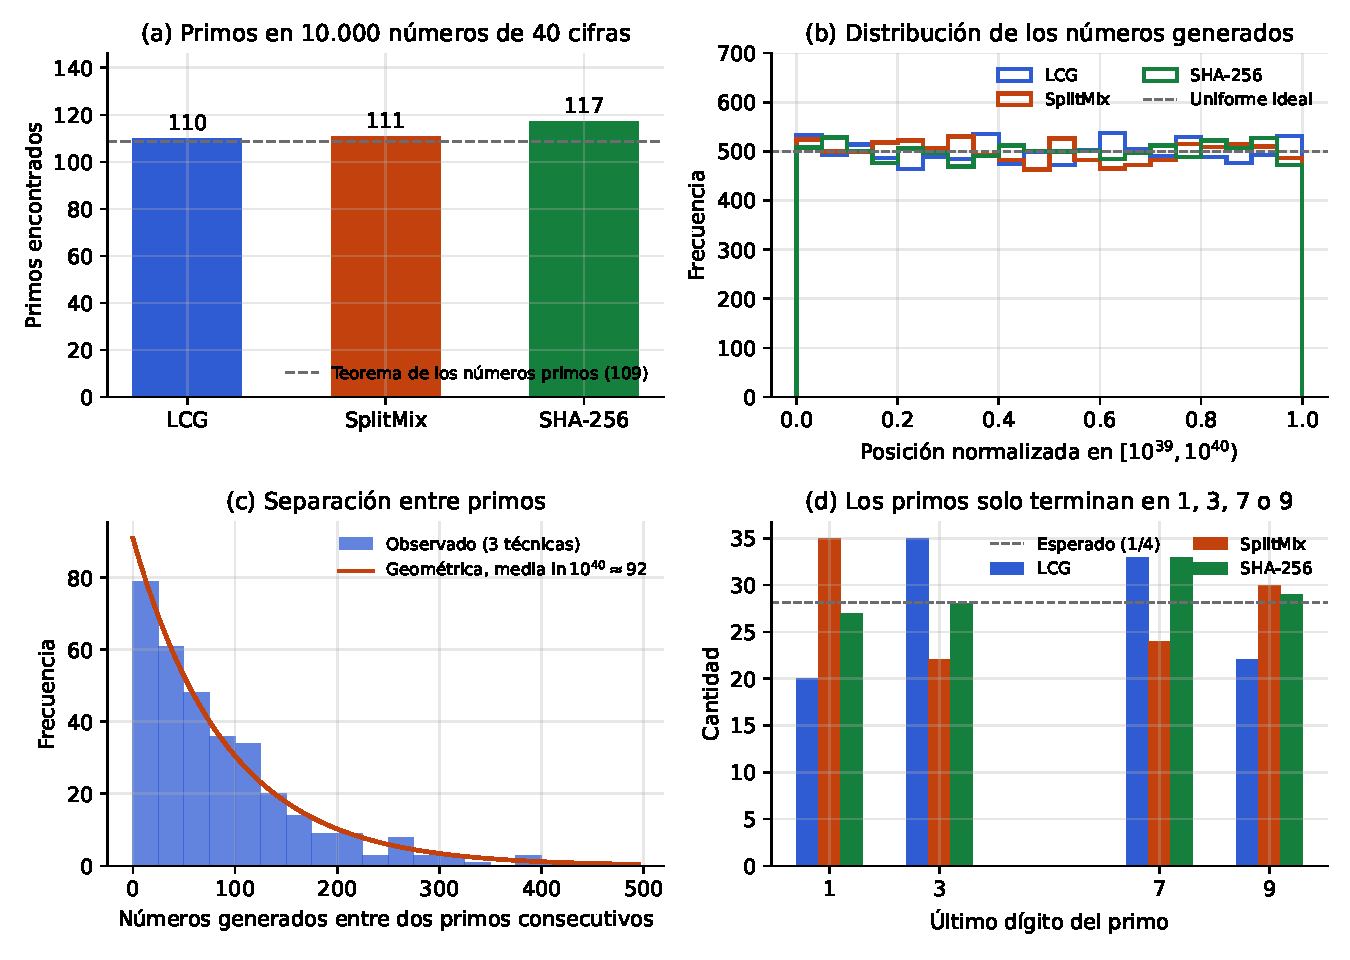
\includegraphics[width=\textwidth]{fig_generacion.pdf}
\caption{Análisis de los 10\,000 números generados por cada técnica.}
\label{fig:gen}
\end{figure}

\begin{itemize}
  \item \textbf{(a)} Por el teorema de los números primos, la probabilidad de
        que un número cercano a $10^{40}$ sea primo es $1/\ln 10^{40} \approx
        1/92$, así que se esperan $\approx 109$ primos. Se obtuvieron 110 (LCG),
        111 (SplitMix) y 117 (SHA-256): diferencias de $+1$\,\%, $+2$\,\% y
        $+8$\,\%, dentro de la variación estadística esperada
        ($\sqrt{109}\approx 10$).
  \item \textbf{(b)} Los números se reparten de forma plana en todo el
        intervalo $[10^{39}, 10^{40})$: ninguna técnica favorece una región.
  \item \textbf{(c)} La cantidad de números entre dos primos consecutivos sigue
        una distribución geométrica con media teórica $92$; las medias
        observadas fueron $90.8$, $90.0$ y $85.3$. Encontrar primos es, en la
        práctica, un proceso aleatorio sin memoria.
  \item \textbf{(d)} Todos los primos terminan en 1, 3, 7 o 9 (un primo mayor
        que 5 no puede ser par ni múltiplo de 5), en proporciones cercanas a
        $1/4$ cada uno.
\end{itemize}

\subsection{Rendimiento del cifrado y descifrado}

\begin{figure}[H]
\centering
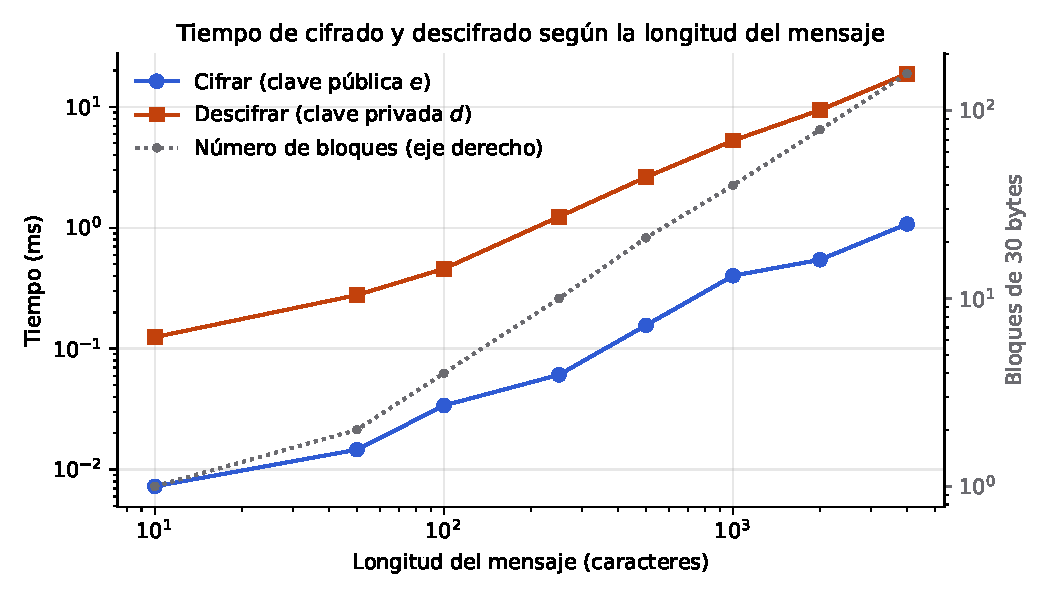
\includegraphics[width=0.8\textwidth]{fig_tiempos_longitud.pdf}
\caption{Tiempo total según la longitud del mensaje (escala log--log).}
\label{fig:long}
\end{figure}

El mensaje se divide en bloques de 30 bytes, de modo que el número de bloques,
y con él el tiempo, crece \textbf{linealmente} con la longitud: un mensaje de
4000 caracteres ocupa 157 bloques y tarda $1.08$\,ms en cifrarse pero
$18.8$\,ms en descifrarse. La Figura~\ref{fig:exp} explica esa diferencia.

\begin{figure}[H]
\centering
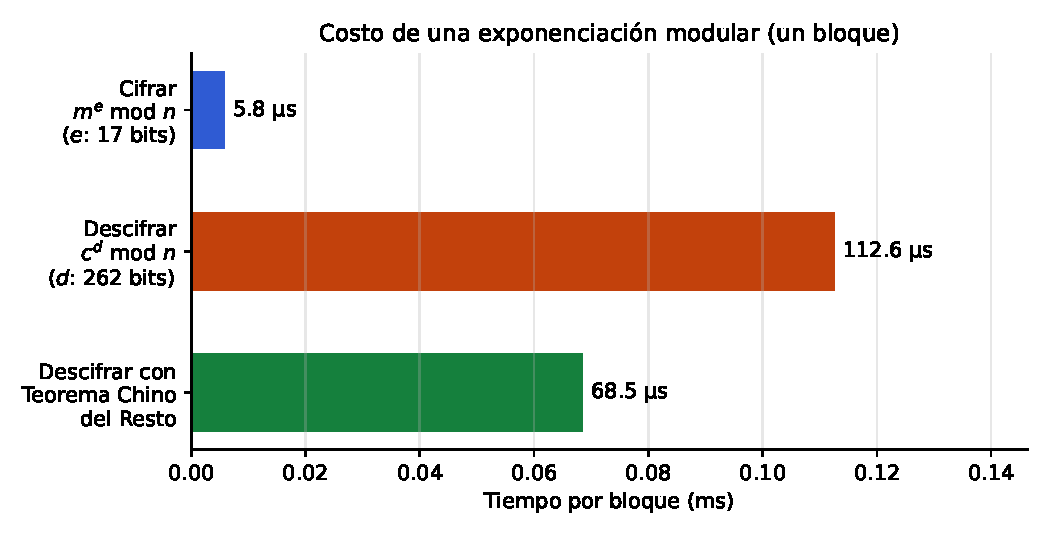
\includegraphics[width=0.75\textwidth]{fig_exponenciacion.pdf}
\caption{Costo de una sola exponenciación modular.}
\label{fig:exp}
\end{figure}

La exponenciación rápida hace una multiplicación por cada bit del exponente y
una adicional por cada bit en 1. El exponente público $e = 65537 = 2^{16}+1$
tiene 17 bits y sólo dos unos, mientras que $d$ tiene 262 bits y 125 unos. Por
eso descifrar ($112.6\,\mu$s) es unas \textbf{20 veces} más lento que cifrar
($5.8\,\mu$s). Aplicando el Teorema Chino del Resto, que trabaja por separado
módulo $p$ y módulo $q$ con exponentes de la mitad de tamaño, el descifrado
baja a $68.5\,\mu$s ($1.6\times$ más rápido) y se obtiene el mismo resultado.
Esta optimización no está en el código original y queda como mejora posible.

\subsection{Calidad del cifrado}

\paragraph{Efecto avalancha.} Se tomaron 1000 mensajes de un bloque y en cada
uno se cambió un único carácter. En el texto plano eso modifica en promedio el
$1.3$\,\% de los bits; en el texto cifrado cambia el
\textbf{49.95\,\%} $\pm$ 3.0\,\%, prácticamente el $50$\,\% ideal
(Figura~\ref{fig:av}). Un cambio mínimo en la entrada produce una salida sin
relación aparente con la anterior: el análogo criptográfico del
\emph{efecto mariposa}.

\begin{figure}[H]
\centering
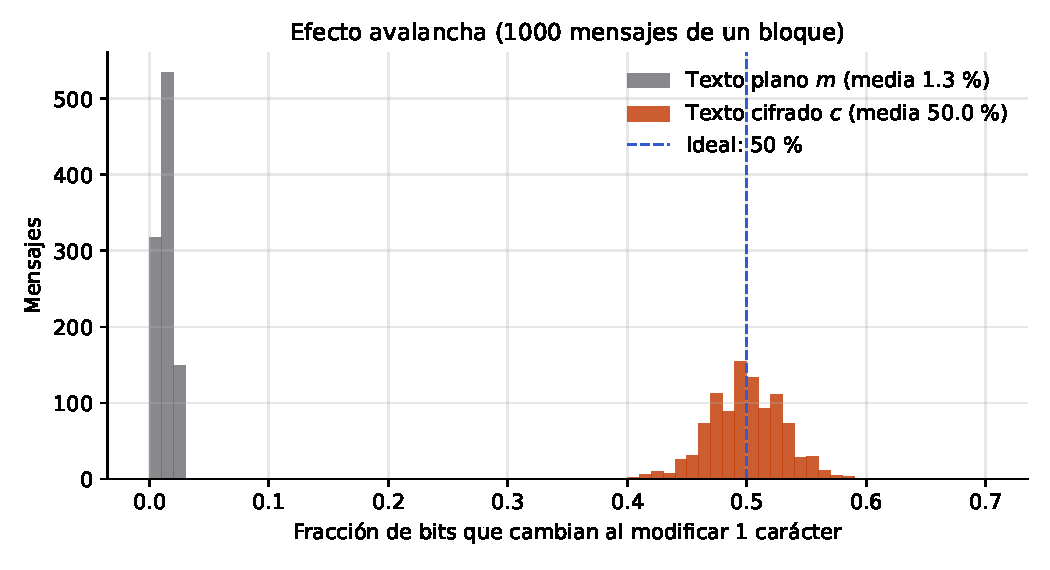
\includegraphics[width=0.78\textwidth]{fig_avalancha.pdf}
\caption{Fracción de bits que cambian al modificar un carácter.}
\label{fig:av}
\end{figure}

\paragraph{Distribución de bytes.} Se cifró el propio \texttt{README.md} del
proyecto (12\,690 bytes, 423 bloques). El texto en español concentra sus bytes
en las letras minúsculas y el espacio, con una entropía de $4.99$ bits/byte.
El texto cifrado es plano en todo el rango 0--255, con $7.99$ de un máximo de
$8$ bits/byte (Figura~\ref{fig:bytes}): no deja ver las frecuencias de letras
que permitirían un análisis estadístico. El costo es una expansión de $10$\,\%,
porque cada bloque de 30 bytes se convierte en un número de 33 bytes.

\begin{figure}[H]
\centering
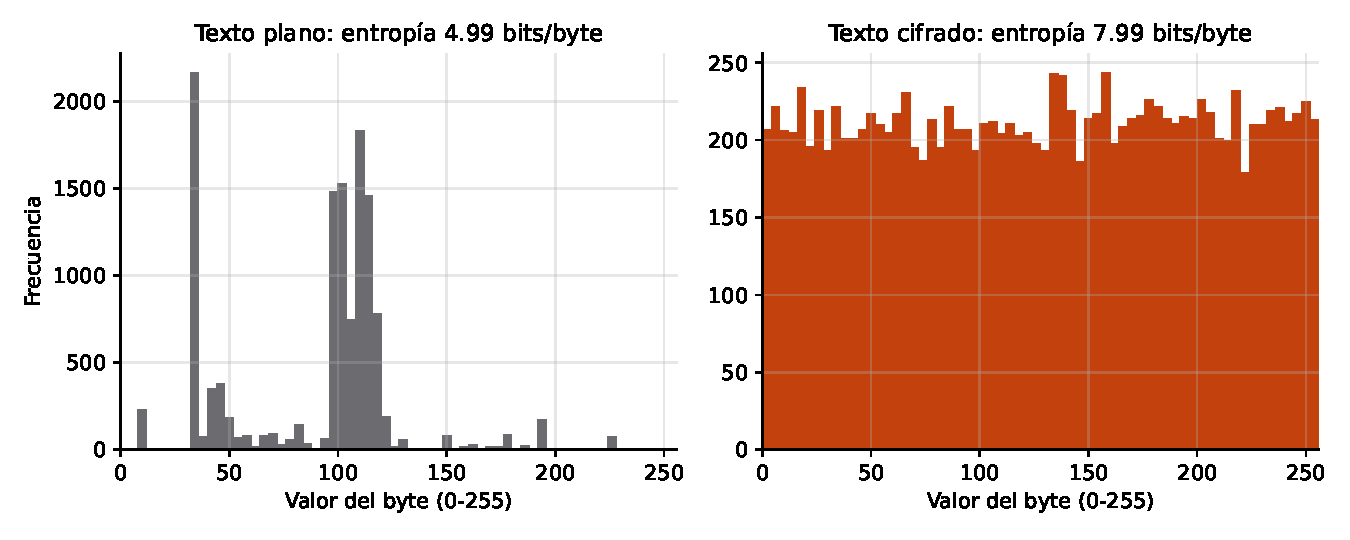
\includegraphics[width=\textwidth]{fig_bytes.pdf}
\caption{Histograma de bytes del texto plano y del texto cifrado (se omite el
byte más significativo de cada bloque, acotado por $n$).}
\label{fig:bytes}
\end{figure}

\subsection{Corrección del sistema}

\begin{table}[H]
\centering
\begin{tabular}{lr}
\toprule
Prueba (1000 mensajes aleatorios, 1--300 caracteres con tildes y ñ) & Resultado \\
\midrule
Recuperados exactamente con la clave correcta & \textbf{1000 / 1000} \\
Recuperados con una clave privada ajena & \textbf{0 / 1000} \\
\quad --- error de decodificación UTF-8 & 962 \\
\quad --- texto basura & 38 \\
\bottomrule
\end{tabular}
\caption{Ida y vuelta del cifrado y descifrado con clave correcta y con clave ajena.}
\end{table}

El sistema es correcto en el 100\,\% de los casos y una clave privada distinta
nunca recupera el mensaje.

\subsection{Seguridad: tamaño de clave y factorización}

\begin{figure}[H]
\centering
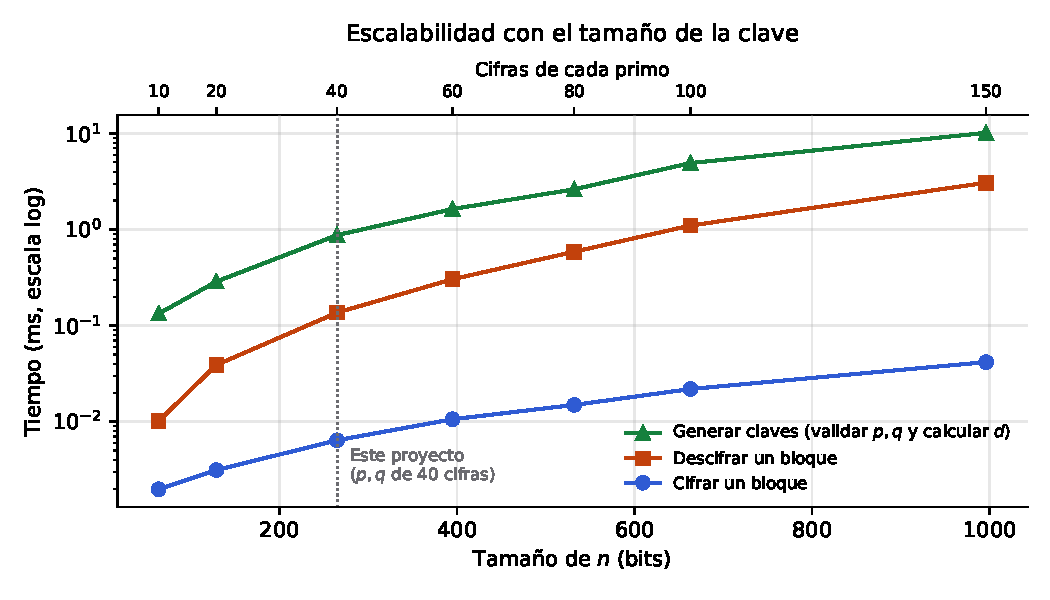
\includegraphics[width=0.8\textwidth]{fig_escalabilidad.pdf}
\caption{Costo de las operaciones según el tamaño de los primos.}
\label{fig:esc}
\end{figure}

Al pasar de primos de 40 a 150 cifras ($n$ de 265 a 996 bits), descifrar un
bloque pasa de $0.14$ a $3.07$\,ms y generar las claves de $0.87$ a
$10.2$\,ms (Figura~\ref{fig:esc}). Para el usuario legítimo, una clave mucho
más grande sigue costando milisegundos.

\begin{figure}[H]
\centering
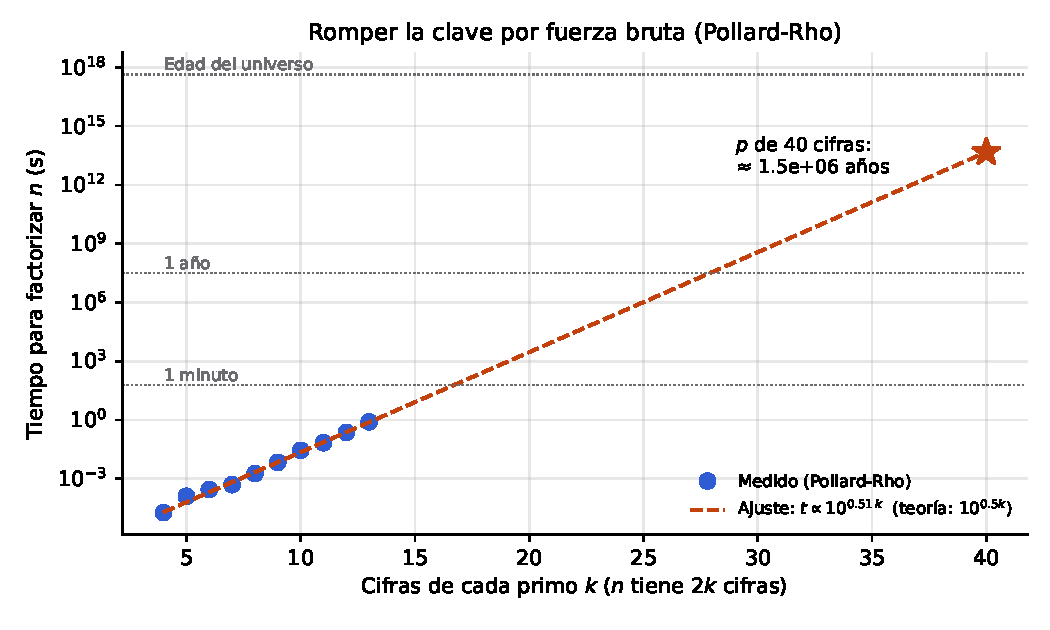
\includegraphics[width=0.8\textwidth]{fig_factorizacion.pdf}
\caption{Tiempo para factorizar $n = pq$ con Pollard-Rho y su extrapolación.}
\label{fig:fac}
\end{figure}

Para un atacante, en cambio, la seguridad de RSA depende de que sea difícil
factorizar $n$. Se implementó el algoritmo Pollard-Rho, cuyo costo esperado es
$O(\sqrt{p})$, y se midió con primos de 4 a 13 cifras. El ajuste da
$t \propto 10^{0.51k}$, casi igual al $10^{0.5k}$ teórico. Con primos de 13
cifras ya tarda $0.8$\,s ($\approx 10^6$ iteraciones); al extrapolar a los 40
cifras del proyecto se obtienen unos $\mathbf{1.5}$ \textbf{millones de años}.

\textbf{Advertencia:} Pollard-Rho no es el mejor ataque. La criba general del
cuerpo de números (GNFS) tiene costo subexponencial y factoriza un $n$ de 80
cifras en poco tiempo con programas como CADO-NFS o msieve. Por eso RSA real
usa $n$ de al menos 2048 bits (617 cifras). La clave de este proyecto es
adecuada para fines didácticos, no para proteger información.

\subsection{Sensibilidad a las condiciones iniciales}

\begin{figure}[H]
\centering
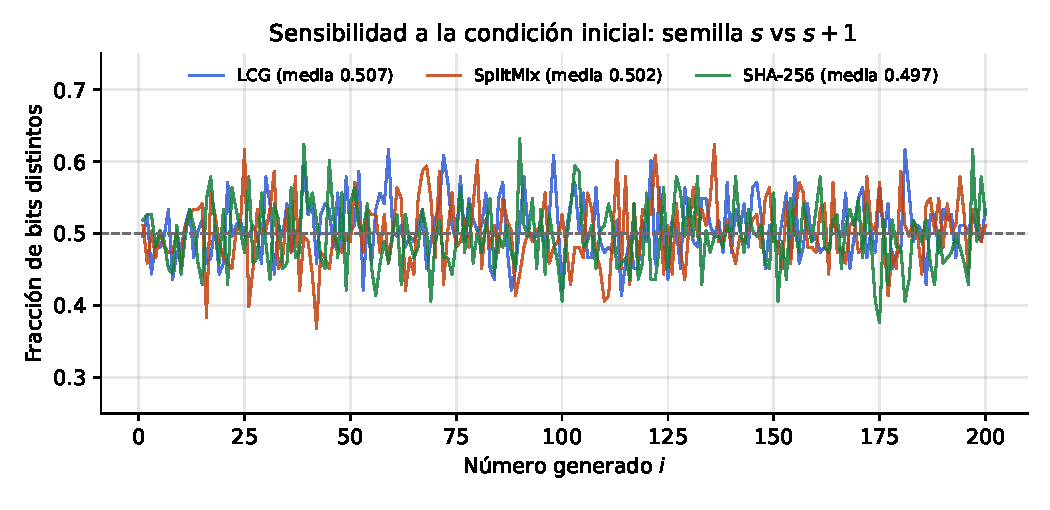
\includegraphics[width=0.8\textwidth]{fig_sensibilidad.pdf}
\caption{Bits distintos entre las secuencias generadas con la semilla $s$ y con $s+1$.}
\label{fig:sens}
\end{figure}

Se generaron 200 números con la semilla 12345 y otros 200 con la semilla 12346.
Desde el primer número, las secuencias difieren en la mitad de sus bits
(medias de $0.507$, $0.502$ y $0.497$). Como en un sistema caótico, una
perturbación mínima de la condición inicial se amplifica por completo, aunque
la regla sea determinista: con la misma semilla se obtienen siempre los mismos
primos y, por tanto, la misma clave.

% =====================================================================
\section{Conclusiones}

\begin{itemize}
  \item \textbf{Generación:} las tres técnicas producen números uniformes de 40
        cifras y entre 110 y 117 primos por cada 10\,000, de acuerdo con el
        teorema de los números primos ($\approx 109$). Los primos aparecen como
        un proceso geométrico, sin memoria.
  \item \textbf{Rendimiento:} el tiempo crece linealmente con el mensaje.
        Descifrar es unas 20 veces más lento que cifrar porque $d$ es mucho más
        grande que $e = 65537$; el Teorema Chino del Resto reduce ese costo en
        $1.6\times$ y es una mejora sencilla de incorporar.
  \item \textbf{Calidad:} el cifrado tiene un efecto avalancha casi ideal
        ($49.95$\,\%) y eleva la entropía de $4.99$ a $7.99$ bits/byte, ocultando
        las frecuencias del idioma.
  \item \textbf{Corrección:} 1000 de 1000 mensajes recuperados y ninguno con
        una clave ajena.
  \item \textbf{Seguridad:} con fuerza bruta (Pollard-Rho) romper la clave
        tomaría millones de años, pero con GNFS un $n$ de 263 bits es
        vulnerable. Además, el RSA ``de libro'' es determinista, ya que un
        mismo mensaje produce siempre el mismo cifrado. En la práctica se usan
        claves de 2048 bits o más, relleno aleatorio (OAEP) y un generador
        criptográficamente seguro.
  \item \textbf{Cibernética y caos:} la máquina es un sistema de comunicación
        Emisor--Canal--Receptor con un lazo de retroalimentación (\texttt{ACK}
        y verificación de integridad), y sus componentes muestran la
        característica central de los sistemas caóticos: reglas deterministas
        simples cuya salida es extremadamente sensible a pequeñas
        perturbaciones, sea en la semilla del generador o en un carácter del
        mensaje.
\end{itemize}

\end{document}
